\documentclass[11pt]{article}

\usepackage[T1]{fontenc}
\usepackage{lmodern}
\usepackage[margin=0.90in]{geometry}
\usepackage{microtype}
\usepackage{amsmath,amssymb,amsthm,mathtools}
\usepackage{booktabs,longtable,array,tabularx}
\usepackage{graphicx}
\usepackage{float}
\usepackage{xcolor}
\usepackage{enumitem}
\usepackage{fancyhdr}
\usepackage{hyperref}
\usepackage[nameinlink,noabbrev]{cleveref}
\usepackage{listings}
\usepackage{caption}
\usepackage{bm}
\usepackage{needspace}
\usepackage{placeins}
\usepackage{siunitx}

\graphicspath{{figures/}}
\allowdisplaybreaks
\sisetup{scientific-notation=true,round-mode=places,round-precision=4}

\hypersetup{
  pdftitle={Projector-Resolved Seed Calculus VIII},
  pdfauthor={Komorebi P.},
  pdfsubject={Packet algorithms, structured operators, complexity and memory bounds, mixed precision, GPU scheduling, fair CPU/GPU benchmarks, and CUDA realization},
  colorlinks=true,
  linkcolor=black,
  citecolor=black,
  urlcolor=black
}

\pagestyle{fancy}
\fancyhf{}
\fancyhead[L]{Projector-Resolved Seed Calculus VIII}
\fancyhead[R]{Komorebi P.}
\fancyfoot[C]{\thepage}
\setlength{\headheight}{14pt}

\newtheorem{theorem}{Theorem}[section]
\newtheorem{proposition}[theorem]{Proposition}
\newtheorem{lemma}[theorem]{Lemma}
\newtheorem{corollary}[theorem]{Corollary}
\theoremstyle{definition}
\newtheorem{definition}[theorem]{Definition}
\newtheorem{example}[theorem]{Example}
\newtheorem{construction}[theorem]{Construction}
\newtheorem{conjecture}[theorem]{Conjecture}
\theoremstyle{remark}
\newtheorem{remark}[theorem]{Remark}
\newtheorem{boundary}[theorem]{Boundary}
\newtheorem{certificate}[theorem]{Numerical Certificate}
\newtheorem{classical}[theorem]{Classical Input}

\newcommand{\cA}{\mathcal A}
\newcommand{\cB}{\mathcal B}
\newcommand{\cC}{\mathcal C}
\newcommand{\cD}{\mathcal D}
\newcommand{\cE}{\mathcal E}
\newcommand{\cF}{\mathcal F}
\newcommand{\cG}{\mathcal G}
\newcommand{\cH}{\mathcal H}
\newcommand{\cK}{\mathcal K}
\newcommand{\cL}{\mathcal L}
\newcommand{\cO}{\mathcal O}
\newcommand{\cP}{\mathcal P}
\newcommand{\cR}{\mathcal R}
\newcommand{\cS}{\mathcal S}
\newcommand{\cT}{\mathcal T}
\newcommand{\bbC}{\mathbb C}
\newcommand{\bbR}{\mathbb R}
\newcommand{\bbN}{\mathbb N}
\newcommand{\Id}{\operatorname{Id}}
\newcommand{\Tr}{\operatorname{Tr}}
\newcommand{\rank}{\operatorname{rank}}
\newcommand{\Ran}{\operatorname{Ran}}
\newcommand{\Ker}{\operatorname{Ker}}
\newcommand{\Spec}{\operatorname{Spec}}
\newcommand{\diag}{\operatorname{diag}}
\newcommand{\cond}{\operatorname{cond}}
\newcommand{\flop}{\operatorname{flop}}
\newcommand{\bytes}{\operatorname{bytes}}
\newcommand{\norm}[1]{\left\lVert#1\right\rVert}
\newcolumntype{L}[1]{>{\raggedright\arraybackslash}p{#1}}
\newcolumntype{Y}{>{\raggedright\arraybackslash}X}

\lstset{
  language=Python,
  basicstyle=\ttfamily\footnotesize,
  breaklines=true,
  frame=single,
  showstringspaces=false,
  columns=fullflexible,
  keepspaces=true,
  numbers=left,
  numberstyle=\tiny,
  numbersep=7pt
}

\title{\textbf{Projector-Resolved Seed Calculus VIII}\\[0.45em]
\large Packet Algorithms and GPU Realization: Dense Operators, Block Transfer, and CUDA}
\author{Komorebi P.}
\date{}

\begin{document}
\maketitle

\begin{abstract}
This paper develops the computational realization of the projector-resolved seed calculus. A finite operator is decomposed into packet blocks $A_{\beta\alpha}=P_\beta A P_\alpha$, and its support graph determines storage, arithmetic, data movement, and scheduling. Exact formulas are proved for block-diagonal, block-sparse, block-diagonal-plus-low-rank, compressed-product, Woodbury-solve, packet-preconditioned Krylov, and mixed-precision computations. For equal block width $b$, rank $r$, dimension $n$, and $q$ right-hand sides, a block-diagonal-plus-low-rank application uses $2qn(b+2r)$ modeled floating-point operations and stores $n(b+2r)$ scalar entries, compared with $2qn^2$ operations and $n^2$ entries for a dense representation. The same reduction factor $n/(b+2r)$ therefore appears in the ideal arithmetic and storage models. A packetwise error theorem bounds mixed-precision reconstruction by block sensitivities, and a continuous allocation theorem assigns tolerances optimally under a declared cost model. Exact amortization thresholds are derived for structure discovery, host-device transfer, compilation, and CUDA Graph capture. The measured corpus contains 154 matched rows from sixteen algorithm suites, comprising 74 CPU and 80 GPU measurements on an RTX 3070 Ti Laptop GPU. The strongest matched structured result is a 14.89-fold speedup over a device-resident GPU dense baseline and a 235.74-fold speedup over the matched CPU dense baseline for an $8192\times8192$ equal-block operator applied to 32 right-hand sides. Negative controls are retained: small Walsh-Hadamard transforms favor the CPU, the tested recursive HODLR GPU path is slower than dense cuBLAS, Strassen is slower than OpenBLAS at the tested sizes, and mixed-precision iterative refinement is slower than a direct FP64 GPU solve in the measured case. Eighteen code-generated figures, a sanitized benchmark corpus, machine-readable results, and twenty-three automated tests accompany the paper. Mathematical complexity statements, measured implementation results, and hardware conjectures are kept separate.
\end{abstract}

\begin{center}
\fbox{\begin{minipage}{0.93\textwidth}
\textbf{Scope and claim boundary.} The paper proves the finite algebraic identities, storage counts, modeled arithmetic counts, error bounds, preconditioner bound, and amortization formulas stated below. Benchmark results are empirical and apply only to the recorded hardware, software, timing scope, output contract, and generated instances. A structure-sensitive algorithm is not compared with generic dense multiplication unless the mathematical output and materialization contract agree. No new generic matrix-multiplication exponent is claimed. Hardware co-design and automatic packet-discovery statements are presented as conjectures or design principles, not as measured facts. Classical references are reserved for the consolidated end-of-series bibliography and are not reproduced here.
\end{minipage}}
\end{center}

\tableofcontents
\listoffigures
\listoftables
\clearpage

\section{The computational seed realization}

The common operator chain becomes
\[
\boxed{
\begin{gathered}
\text{data seed}
\longrightarrow
\text{packet address}
\longrightarrow
\text{structured operator}\\
\longrightarrow
\text{hardware schedule}
\longrightarrow
\text{error certificate}
\longrightarrow
\text{reconstruction}
\end{gathered}
}
\]

\begin{figure}[htbp]
\centering
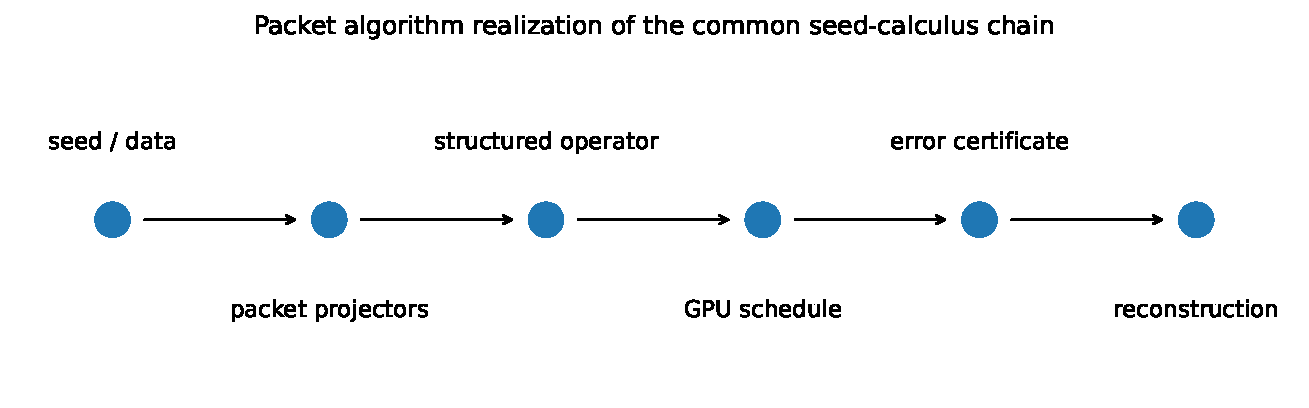
\includegraphics[width=0.98\textwidth]{01_packet_gpu_architecture.pdf}
\caption{The computational realization of the seed calculus. The mathematical packet representation is fixed before the CPU or GPU implementation is selected.}
\label{fig:architecture}
\end{figure}

\begin{definition}[Finite packet operator]
Let $X=\bigoplus_{\alpha\in I}X_\alpha$ with complete idempotents
\[
P_\alpha P_\beta=\delta_{\alpha\beta}P_\alpha,
\qquad
\sum_{\alpha\in I}P_\alpha=I.
\]
For $A:X\to X$, define the packet block
\[
A_{\beta\alpha}=P_\beta A P_\alpha:X_\alpha\to X_\beta.
\]
The directed support graph $G_A$ has vertex set $I$ and an edge $\alpha\to\beta$ whenever $A_{\beta\alpha}\neq0$.
\end{definition}

\begin{theorem}[Exact packet reconstruction]
Every finite packet operator satisfies
\[
\boxed{
A=\sum_{\alpha,\beta\in I}A_{\beta\alpha}.
}
\]
For any matrix of right-hand sides $X$,
\[
\boxed{
AX=\sum_{\beta}\sum_{\alpha}A_{\beta\alpha}P_\alpha X.
}
\]
\end{theorem}

\begin{proof}
Insert the identity on both sides of $A$:
\[
A=\left(\sum_\beta P_\beta\right)A\left(\sum_\alpha P_\alpha\right)
 =\sum_{\alpha,\beta}P_\beta AP_\alpha.
\]
Applying the identity to $X$ gives the second formula.
\end{proof}

The operator may be written as
\[
A=D+K,
\qquad
D=\sum_\alpha A_{\alpha\alpha},
\qquad
K=\sum_{\alpha\neq\beta}A_{\beta\alpha}.
\]
Here $D$ contains packet-preserving work and $K$ contains transfers. The computational problem is determined not only by $n=\dim X$, but by the block dimensions, support graph, ranks of cross-packet transfers, right-hand-side count, output contract, and reuse count.

\begin{figure}[htbp]
\centering
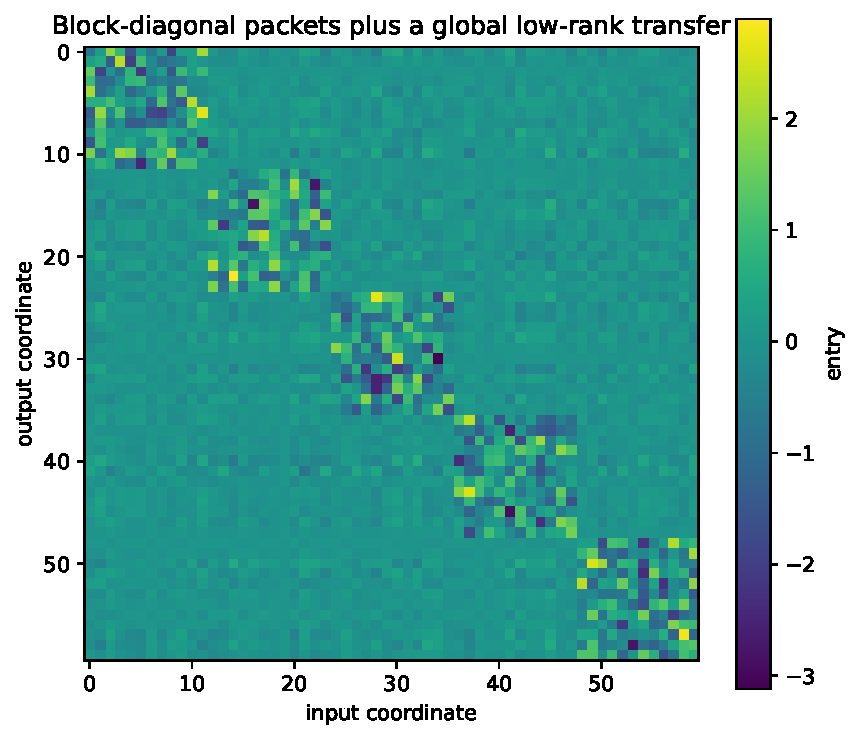
\includegraphics[width=0.72\textwidth]{02_bdlr_structure.pdf}
\caption{A block-diagonal packet operator with a global low-rank transfer. Dense appearance does not imply dense representation cost.}
\label{fig:bdlr-structure}
\end{figure}

\section{Arithmetic and storage models}

Let $n_\alpha=\dim X_\alpha$, $n=\sum_\alpha n_\alpha$, and let $q$ be the number of right-hand sides. We count one multiplication and one addition as two modeled floating-point operations. Lower-order boundary terms are omitted from the count, as in standard matrix-multiplication models.

\begin{theorem}[Dense and packet apply counts]
A dense $n\times n$ operator applied to $q$ right-hand sides has modeled cost
\[
\boxed{
\flop_{\mathrm{dense}}=2n^2q.
}
\]
A packet operator supported on edge set $E\subset I\times I$ has modeled cost
\[
\boxed{
\flop_{\mathrm{packet}}
 =2q\sum_{(\beta,\alpha)\in E}n_\beta n_\alpha.
}
\]
The corresponding representation stores
\[
\boxed{
M_{\mathrm{packet}}
 =\sum_{(\beta,\alpha)\in E}n_\beta n_\alpha
}
\]
scalar entries.
\end{theorem}

\begin{proof}
The block $A_{\beta\alpha}$ is an $n_\beta\times n_\alpha$ matrix. Multiplication by an $n_\alpha\times q$ right-hand side requires $2n_\beta n_\alpha q$ modeled operations and stores $n_\beta n_\alpha$ scalars. Summing over active edges gives both formulas.
\end{proof}

\begin{corollary}[Equal block-diagonal packets]
If $n$ is partitioned into $n/b$ equal blocks of width $b$, then
\[
\flop_{\mathrm{block}}=2qnb,
\qquad
M_{\mathrm{block}}=nb.
\]
The ideal dense-to-block reduction is
\[
\boxed{
\frac{n^2}{nb}=\frac{n}{b}.
}
\]
\end{corollary}

\begin{definition}[Block diagonal plus low rank]
A BDLR operator has the form
\[
\boxed{
A=D+UV^*,
}
\]
where $D=\bigoplus_\alpha D_\alpha$, $U,V\in\bbC^{n\times r}$, and $r\ll n$.
\end{definition}

\begin{theorem}[BDLR apply and storage]
For $q$ right-hand sides,
\[
AX=DX+U(V^*X)
\]
has modeled cost
\[
\boxed{
\flop_{\mathrm{BDLR}}
 =2q\left(\sum_\alpha n_\alpha^2+2nr\right),
}
\]
and stores
\[
\boxed{
M_{\mathrm{BDLR}}
 =\sum_\alpha n_\alpha^2+2nr
}
\]
scalars. For equal block width $b$,
\[
\boxed{
\flop_{\mathrm{BDLR}}=2qn(b+2r),
\qquad
M_{\mathrm{BDLR}}=n(b+2r).
}
\]
Thus the ideal dense-to-BDLR reduction factor is
\[
\boxed{
S_{\mathrm{ideal}}=\frac{n}{b+2r}.
}
\]
\end{theorem}

\begin{proof}
The block-diagonal product costs $2q\sum_\alpha n_\alpha^2$. The product $V^*X$ costs $2nrq$, and multiplication of the resulting $r\times q$ matrix by $U$ costs another $2nrq$. Storage consists of the diagonal blocks and the two rank factors. For equal blocks, $\sum_\alpha n_\alpha^2=(n/b)b^2=nb$.
\end{proof}

\begin{certificate}[Model case]
For $n=8192$, $b=64$, $r=8$, and $q=32$,
\[
\flop_{\mathrm{dense}}=4{,}294{,}967{,}296,
\qquad
\flop_{\mathrm{BDLR}}=41{,}943{,}040.
\]
In FP32, dense storage is $268{,}435{,}456$ bytes, while the BDLR representation requires $2{,}621{,}440$ bytes. Both ideal reduction factors equal
\[
\boxed{102.4.}
\]
This is an arithmetic and representation statement; measured speedup is smaller because launches, memory traffic, and hardware occupancy remain.
\end{certificate}

\begin{figure}[htbp]
\centering
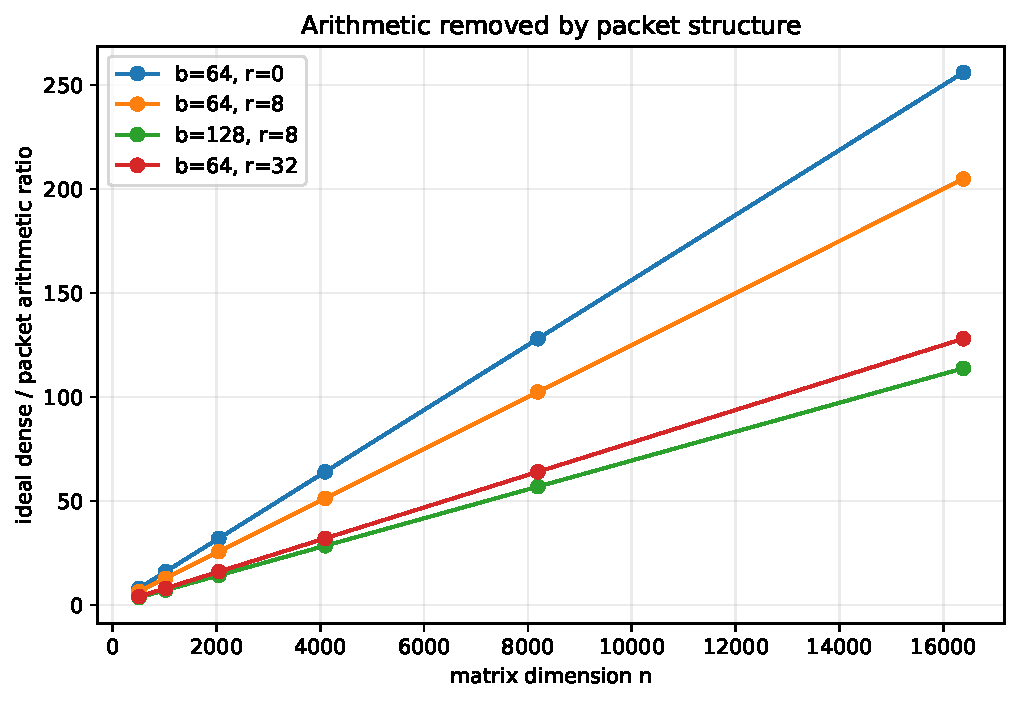
\includegraphics[width=0.78\textwidth]{03_ideal_packet_speedup.pdf}
\caption{Ideal arithmetic reduction for equal packet width and low-rank transfer. The benefit grows with $n$ only when $b$ and $r$ remain controlled.}
\label{fig:ideal-speedup}
\end{figure}

\begin{figure}[htbp]
\centering
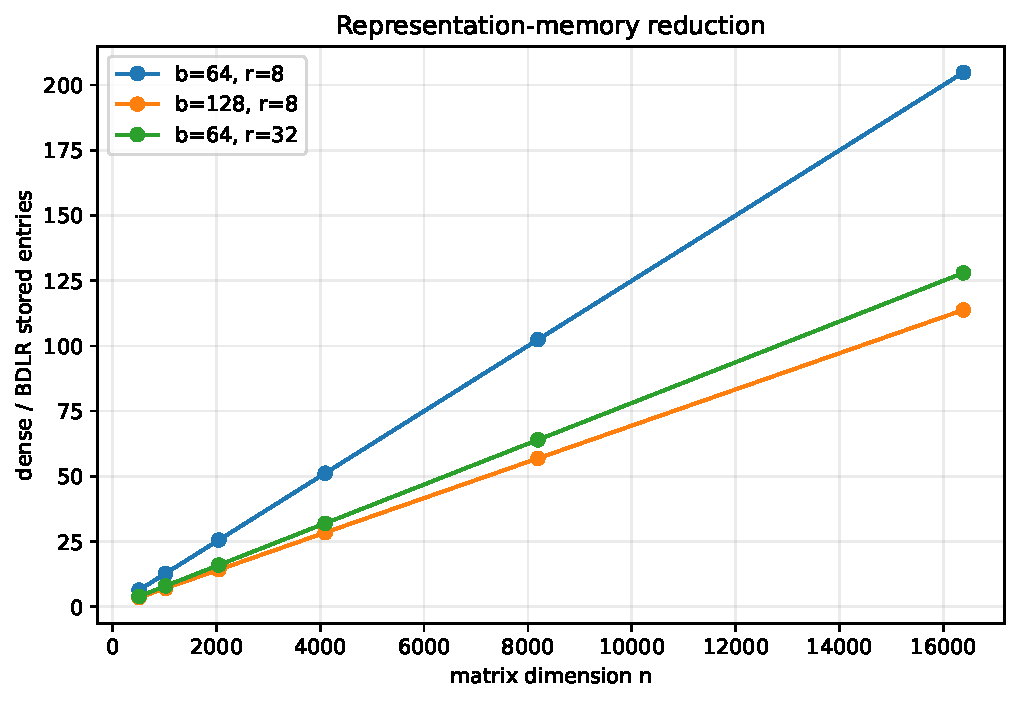
\includegraphics[width=0.78\textwidth]{04_representation_memory_reduction.pdf}
\caption{Dense-to-BDLR representation-memory reduction. A structure-sensitive method changes the stored mathematical object before changing the hardware.}
\label{fig:memory-reduction}
\end{figure}

\section{Exact BDLR algebra}

\subsection{Compressed products}

Let
\[
A=D_A+U_AV_A^*,
\qquad
B=D_B+U_BV_B^*,
\]
with the same diagonal packet partition.

\begin{proposition}[Exact compressed BDLR product]
The product $AB$ is represented exactly as
\[
AB=D_AD_B+U_CV_C^*,
\]
where
\[
U_C=
\begin{bmatrix}
D_AU_B+U_A(V_A^*U_B) & U_A
\end{bmatrix},
\]
\[
V_C=
\begin{bmatrix}
V_B & D_B^*V_A
\end{bmatrix}.
\]
Its unrecompressed rank is at most $r_A+r_B$.
\end{proposition}

\begin{proof}
Expand:
\[
AB=D_AD_B+D_AU_BV_B^*+U_AV_A^*D_B+U_A(V_A^*U_B)V_B^*.
\]
The second and fourth terms combine as
\[
\left(D_AU_B+U_A(V_A^*U_B)\right)V_B^*,
\]
and
\[
U_AV_A^*D_B=U_A(D_B^*V_A)^*.
\]
Concatenating the two low-rank terms gives the formula.
\end{proof}

The compressed output is not the same output contract as a materialized $n\times n$ matrix. If the downstream computation accepts BDLR factors, materialization is unnecessary. If it requires every matrix entry, the cost of materialization must be included.

\begin{figure}[htbp]
\centering
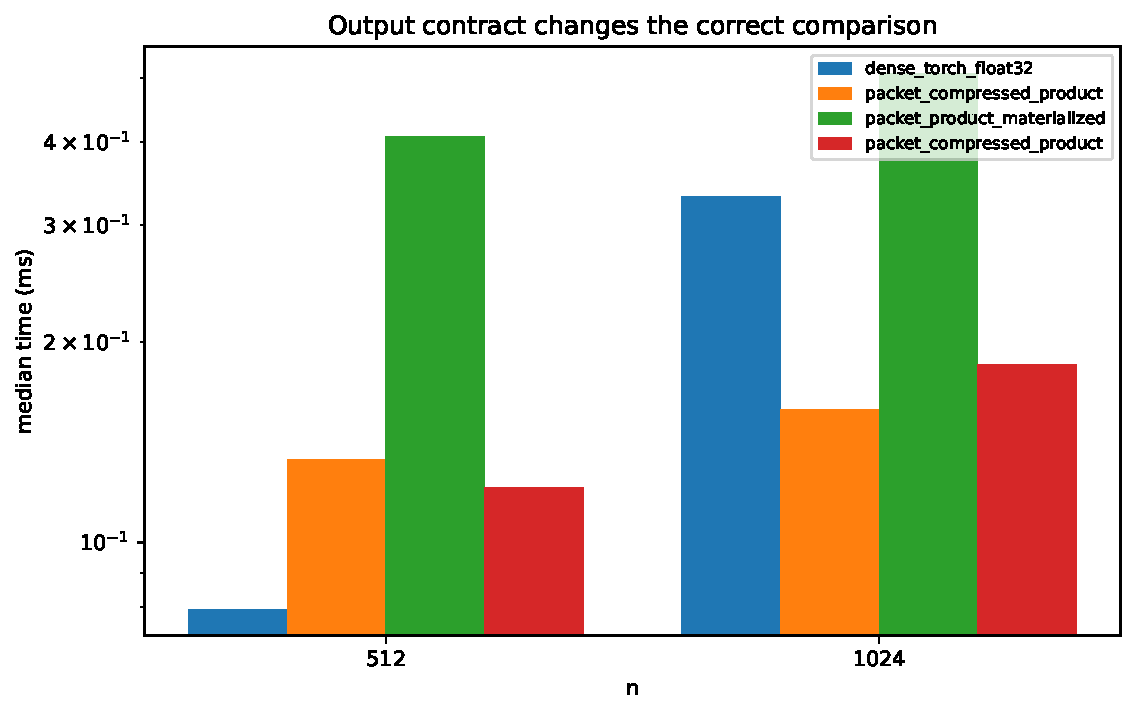
\includegraphics[width=0.82\textwidth]{09_compressed_vs_materialized.pdf}
\caption{Measured BDLR product timings. Compressed and explicit outputs answer different computational questions and therefore are not ranked directly against one another.}
\label{fig:compressed-materialized}
\end{figure}

\subsection{Woodbury packet solve}

\begin{theorem}[Exact BDLR inverse]
Assume $D$ and $I_r+V^*D^{-1}U$ are invertible. Then
\[
\boxed{
(D+UV^*)^{-1}
 =D^{-1}-D^{-1}U(I_r+V^*D^{-1}U)^{-1}V^*D^{-1}.
}
\]
\end{theorem}

\begin{proof}
Set
\[
W=D^{-1}-D^{-1}U(I_r+V^*D^{-1}U)^{-1}V^*D^{-1}.
\]
Multiplying $(D+UV^*)W$ and collecting the coefficient of $V^*D^{-1}$ gives
\[
U-U(I_r+V^*D^{-1}U)(I_r+V^*D^{-1}U)^{-1}=0.
\]
The remaining term is the identity. The right inverse calculation is analogous.
\end{proof}

The large solve is reduced to independent packet solves with $D_\alpha$ and one dense $r\times r$ solve. The finite verification gave a residual of
\[
1.62\times10^{-15}.
\]

\section{Block-sparse transfer graphs}

A block-sparse operator is determined by a support graph $E$. The graph supplies both a mathematical sparsity pattern and a GPU scheduling problem.

\begin{theorem}[Path support of powers]
If $A_{\beta\alpha}=0$ whenever $(\beta,\alpha)\notin E$, then
\[
P_\gamma A^mP_\alpha
\]
is a sum over directed paths
\[
\alpha=\alpha_0\to\alpha_1\to\cdots\to\alpha_m=\gamma
\]
in $G_A$, with path contribution
\[
A_{\alpha_m\alpha_{m-1}}\cdots A_{\alpha_1\alpha_0}.
\]
If no such path exists, $P_\gamma A^mP_\alpha=0$.
\end{theorem}

\begin{proof}
Insert the packet identity between every two factors of $A$. Every summand is indexed by an intermediate packet sequence. A factor vanishes unless its corresponding graph edge is active.
\end{proof}

This theorem separates a block-banded operator, a sparse transfer graph, and a recursively nested HODLR operator. They may have similar storage counts but very different launch and indexing costs.

\begin{remark}[Regularity matters]
Equal-size blocks with a regular support pattern map naturally to batched matrix multiplication. Irregular edges require gather/scatter or grouped kernels. Recursive HODLR traversal may produce many small launches and poor utilization. Structure alone does not guarantee a fast GPU realization.
\end{remark}

\section{Packet Krylov and preconditioning}

Let $A=D+K$ be Hermitian positive definite, with $D$ block diagonal and positive definite.

\begin{theorem}[Block-Jacobi condition bound]\label{thm:preconditioner}
Suppose
\[
E=D^{-1/2}KD^{-1/2}
\]
is Hermitian and
\[
\norm{E}_2\le\eta<1.
\]
Then every eigenvalue of
\[
D^{-1/2}AD^{-1/2}=I+E
\]
lies in $[1-\eta,1+\eta]$, and
\[
\boxed{
\cond_2(D^{-1/2}AD^{-1/2})
\le
\frac{1+\eta}{1-\eta}.
}
\]
\end{theorem}

\begin{proof}
For every unit vector $x$,
\[
|x^*Ex|\le\norm{E}_2\le\eta.
\]
Thus the Rayleigh quotient of $I+E$ lies between $1-\eta$ and $1+\eta$. The condition-number bound follows from the ratio of the largest and smallest eigenvalue bounds.
\end{proof}

The finite model had $\eta=0.02943$, yielding the bound
\[
\cond_2\le1.06064.
\]
Conjugate gradient required 31 iterations without preconditioning and 6 iterations with the exact packet block-Jacobi solve.

\begin{figure}[htbp]
\centering
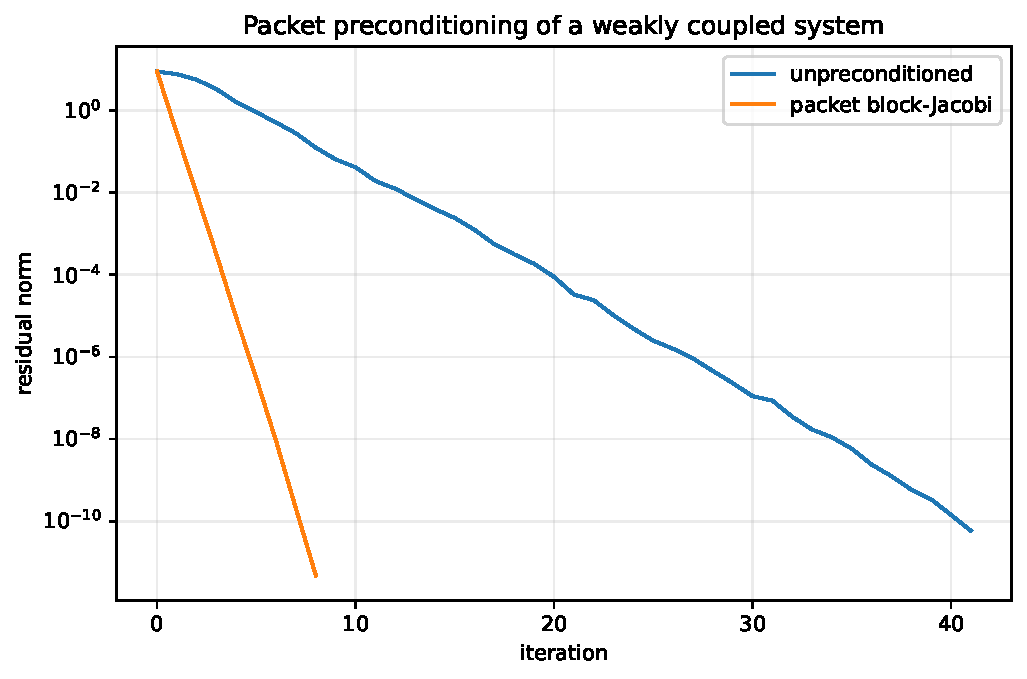
\includegraphics[width=0.78\textwidth]{17_packet_preconditioner.pdf}
\caption{Residual histories for a weakly coupled positive system. The block-diagonal packet operator is used as an exact local preconditioner.}
\label{fig:preconditioner}
\end{figure}

\begin{proposition}[Invariant packet Krylov decomposition]
If $[A,P_\alpha]=0$ for every packet and $v=\sum_\alpha v_\alpha$, then
\[
\cK_m(A,v)
\subseteq
\bigoplus_\alpha\cK_m(A_\alpha,v_\alpha),
\qquad
A_\alpha=P_\alpha AP_\alpha.
\]
Moreover,
\[
A^jv=\sum_\alpha A_\alpha^jv_\alpha
\]
for every $j\ge0$.
\end{proposition}

\begin{proof}
Commutation implies $AP_\alpha=P_\alpha A$ and therefore $A^jP_\alpha=P_\alpha A^j$. Hence
\[
A^jv=\sum_\alpha A^jP_\alpha v
      =\sum_\alpha P_\alpha A^jv
      =\sum_\alpha A_\alpha^jv_\alpha.
\]
Taking spans proves the inclusion.
\end{proof}

\section{Packetwise mixed precision}

The precision decision should be attached to packet transfers rather than selected globally by one dtype whenever packet sensitivities differ.

\begin{theorem}[Packet error certificate]
Let
\[
A=\sum_{e\in E}A_e,
\qquad
\widehat A=\sum_{e\in E}(A_e+E_e),
\]
and suppose edge $e$ originates in packet $\alpha(e)$. Then
\[
\boxed{
\norm{(\widehat A-A)x}
\le
\sum_{e\in E}\norm{E_e}\,\norm{P_{\alpha(e)}x}.
}
\]
If
\[
\norm{E_e}\le\varepsilon_e\norm{A_e},
\]
then
\[
\boxed{
\norm{(\widehat A-A)x}
\le
\sum_{e\in E}
\varepsilon_e\norm{A_e}\,\norm{P_{\alpha(e)}x}.
}
\]
\end{theorem}

\begin{proof}
Use exact reconstruction and the triangle inequality:
\[
(\widehat A-A)x=\sum_eE_eP_{\alpha(e)}x.
\]
Taking norms gives the result.
\end{proof}

In the finite mixed-precision test, the actual error was
\[
1.2614\times10^{-2},
\]
while the certified bound was
\[
2.4605\times10^{-2}.
\]

\begin{theorem}[Continuous precision allocation]
Let $s_e>0$ be packet sensitivities and $c_e>0$ packet costs. In the idealized model
\[
\min_{\varepsilon_e>0}
\sum_e c_e\log\frac1{\varepsilon_e}
\quad\text{subject to}\quad
\sum_es_e\varepsilon_e=\tau,
\]
the unique stationary minimizer is
\[
\boxed{
\varepsilon_e
 =\frac{\tau c_e}{s_e\sum_f c_f}.
}
\]
\end{theorem}

\begin{proof}
The Lagrangian derivative is
\[
-\frac{c_e}{\varepsilon_e}+\lambda s_e=0,
\]
so $\varepsilon_e=c_e/(\lambda s_e)$. Imposing the constraint gives
\[
\lambda=\frac{\sum_fc_f}{\tau}.
\]
Strict convexity in $-\log\varepsilon_e$ gives uniqueness within the feasible positive region.
\end{proof}

\begin{figure}[htbp]
\centering
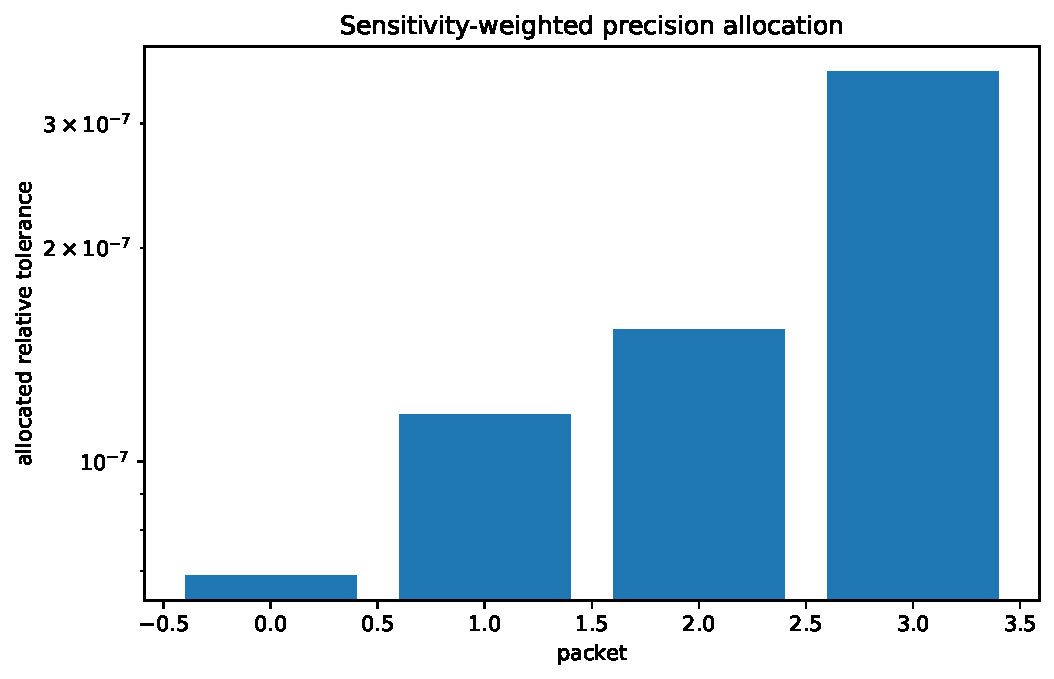
\includegraphics[width=0.76\textwidth]{16_precision_allocation.pdf}
\caption{An example of sensitivity-weighted packet tolerances. More sensitive packets receive tighter error budgets.}
\label{fig:precision-allocation}
\end{figure}

\begin{boundary}[Discrete dtypes]
The theorem solves a continuous model. Mapping its tolerances to FP64, FP32, TF32, BF16, FP16, or custom formats is a discrete scheduling problem and must respect underflow, overflow, accumulation dtype, and kernel availability.
\end{boundary}

\section{GPU mapping of packet operators}

\subsection{Shape classes and batched kernels}

Suppose $B$ independent packet blocks share the same shape. Executing each block with a separate launch requires $B$ launches. Stacking them into a three-dimensional array permits one batched launch.

\begin{proposition}[Shape-class launch reduction]
If packet blocks fall into $g$ distinct shape classes, grouping by shape reduces the launch count from the number of blocks $B$ to at most $g$ without changing the arithmetic or mathematical output.
\end{proposition}

\begin{proof}
Blocks in one shape class may be placed along a batch dimension and passed to a batched matrix multiplication. Each block still receives the same operands and produces the same output block. One launch is required per shape class.
\end{proof}

This explains why equal block-diagonal multiplication maps efficiently to \texttt{bmm}, while irregular block-banded and HODLR paths require more careful fusion.

\subsection{Device residency and transfer}

Let $t_C$ be CPU time, $t_G$ device-resident GPU time, and $t_T$ one-time transfer cost amortized across $R$ uses.

\begin{theorem}[Transfer amortization threshold]
If $t_C>t_G$, the GPU path is faster after $R$ reuses whenever
\[
\boxed{
R>\frac{t_T}{t_C-t_G}.
}
\]
The smallest integer reuse count is
\[
\boxed{
R_{\min}
 =\left\lfloor\frac{t_T}{t_C-t_G}\right\rfloor+1.
}
\]
If $t_C\le t_G$, no reuse count can amortize a positive transfer cost.
\end{theorem}

\begin{proof}
The inequality $t_T+Rt_G<Rt_C$ is equivalent to $R(t_C-t_G)>t_T$.
\end{proof}

The same formula applies to structure discovery, compilation, or graph capture by replacing $t_T$ with the relevant one-time setup cost.

\begin{corollary}[CUDA Graph break-even]
If graph capture costs $c$, ordinary launches cost $t_o$ per use, and replay costs $t_r<t_o$, then graph capture is amortized when
\[
R>\frac{c}{t_o-t_r}.
\]
\end{corollary}

\subsection{Output contracts}

\begin{definition}[Output contract]
An output contract declares the mathematical object returned by an algorithm. Examples include:
\begin{itemize}[leftmargin=1.4em]
\item an explicit matrix;
\item an explicit vector or matrix of right-hand sides;
\item block and low-rank factors;
\item spectral factors;
\item an implicit callable operator.
\end{itemize}
Two timings are directly rankable only when their output contracts agree, or when the cost of converting one output to the other is included.
\end{definition}

\begin{definition}[Timing scope]
A timing scope declares whether the measurement includes device-resident kernels, graph replay, host-to-device transfer, device-to-host transfer, compilation, structure discovery, or materialization.
\end{definition}

\begin{figure}[htbp]
\centering
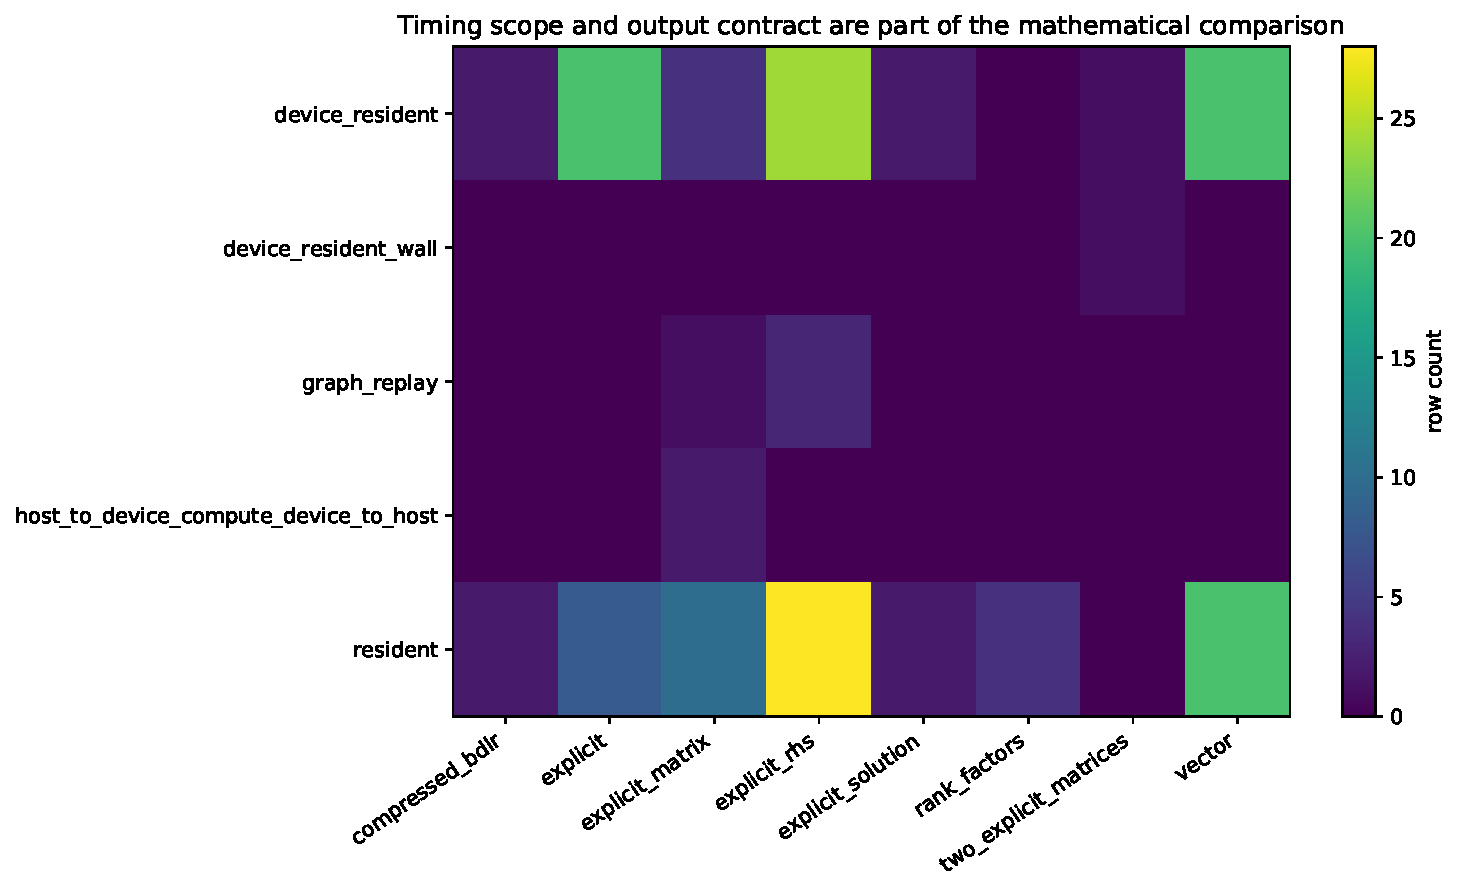
\includegraphics[width=0.92\textwidth]{18_benchmark_contracts.pdf}
\caption{The measured corpus contains several timing scopes and output contracts. These labels are part of the mathematical comparison, not decorative metadata.}
\label{fig:contracts}
\end{figure}

\section{Benchmark protocol and measured corpus}

\subsection{Fairness rules}

The benchmark analysis enforces the following rules:
\begin{enumerate}[leftmargin=1.6em]
\item comparisons occur inside one generated case identifier;
\item dimensions, packet width, rank, right-hand sides, source dtype, and random seed agree;
\item the output contract agrees;
\item the correctness reference is shared;
\item the timing scope is reported;
\item compressed outputs are not ranked against explicit outputs without materialization;
\item negative results are retained.
\end{enumerate}

The automated audit found no fairness-group violations in the sanitized corpus.

\subsection{Recorded environment}

The measured dataset contains 154 rows from sixteen suites:
\[
74\text{ CPU measurements},
\qquad
80\text{ GPU measurements}.
\]
All rows have status \texttt{measured}. The recorded GPU is an NVIDIA GeForce RTX 3070 Ti Laptop GPU with compute capability 8.6, 8~GB nominal memory, and 46 streaming multiprocessors. PyTorch 2.11.0 was built against CUDA 12.8. The CPU environment reports 20 logical cores and a 20-thread OpenBLAS pool.

\begin{table}[htbp]
\centering
\caption{Measured suite coverage.}
\label{tab:suites}
\begin{tabular}{lr@{\qquad}lr}
\toprule
Suite & Rows & Suite & Rows\\
\midrule
Dense GEMM & 28 & BDLR application & 15\\
Block diagonal & 12 & BDLR product & 12\\
Circulant & 12 & Toeplitz & 12\\
Kronecker & 12 & Block banded & 8\\
Sparse plus low rank & 8 & HODLR & 8\\
Strassen & 6 & Transfer pipeline & 5\\
Walsh-Hadamard & 4 & Hidden blocks & 4\\
Randomized low rank & 4 & Iterative refinement & 4\\
\bottomrule
\end{tabular}
\end{table}

\begin{boundary}[Hardware specificity]
The finite correctness tests were rerun in the release environment. The GPU timings themselves come from the supplied measured corpus and were not regenerated on an unreported accelerator. They establish performance on the recorded machine, not on all GPUs.
\end{boundary}

\section{Dense baselines and the precision frontier}

\begin{figure}[htbp]
\centering
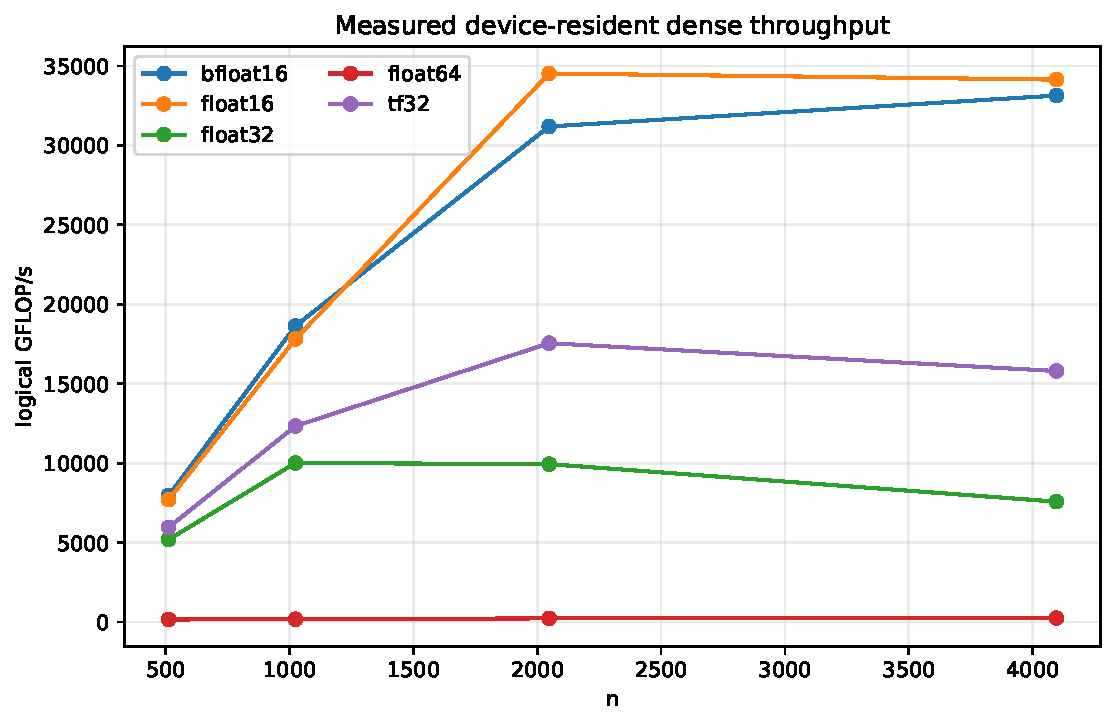
\includegraphics[width=0.82\textwidth]{05_dense_gpu_throughput.pdf}
\caption{Measured device-resident dense throughput across sizes and dtypes. Logical GFLOP/s is based on the dense arithmetic count.}
\label{fig:dense-throughput}
\end{figure}

For the $4096\times4096$ float32-source case, the measured device-resident results were:

\begin{table}[htbp]
\centering
\caption{Dense GPU precision frontier at $n=4096$.}
\label{tab:dense-frontier}
\begin{tabular}{lrrr}
\toprule
Method & Median (ms) & Logical GFLOP/s & Relative error\\
\midrule
FP32 & 18.1309 & 7580.35 & $5.76\times10^{-7}$\\
TF32 & 8.6999 & 15797.75 & $2.94\times10^{-4}$\\
FP16 & 4.0264 & 34134.72 & $3.60\times10^{-4}$\\
BF16 & 4.1482 & 33132.00 & $2.88\times10^{-3}$\\
\bottomrule
\end{tabular}
\end{table}

The comparison is not a universal ranking of dtypes. It is a measured accuracy-throughput frontier for one generated family. FP16 was 4.50 times faster than the matched FP32 GPU row, while BF16 had the largest error in the corpus.

\begin{figure}[htbp]
\centering
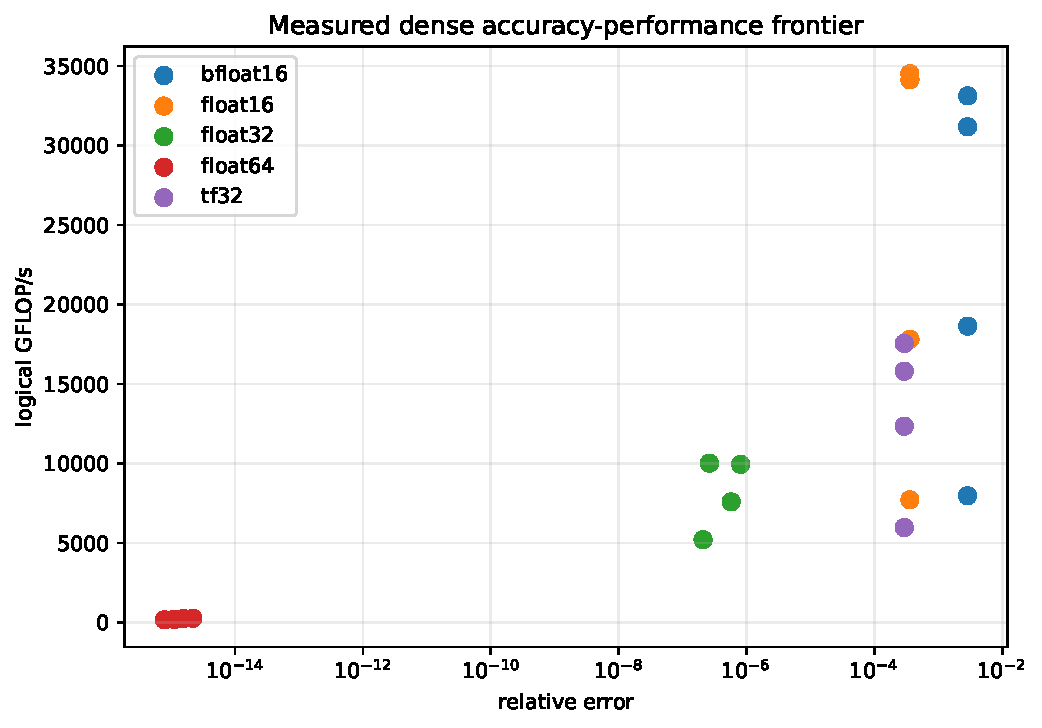
\includegraphics[width=0.80\textwidth]{06_accuracy_performance_frontier.pdf}
\caption{Measured dense accuracy-performance points. A packet precision policy should select among such local frontiers according to packet sensitivity.}
\label{fig:accuracy-frontier}
\end{figure}

\section{Measured structured operators}

\subsection{Equal block diagonal}

For $n=8192$, $b=64$, and 32 right-hand sides, the device-resident batched packet method took
\[
0.046032\text{ ms}.
\]
It was
\[
\boxed{14.8919\times}
\]
faster than the matched device-resident GPU dense row and
\[
\boxed{235.7404\times}
\]
faster than the matched CPU dense row. Its relative error was
\[
8.17\times10^{-8}.
\]

\begin{figure}[htbp]
\centering
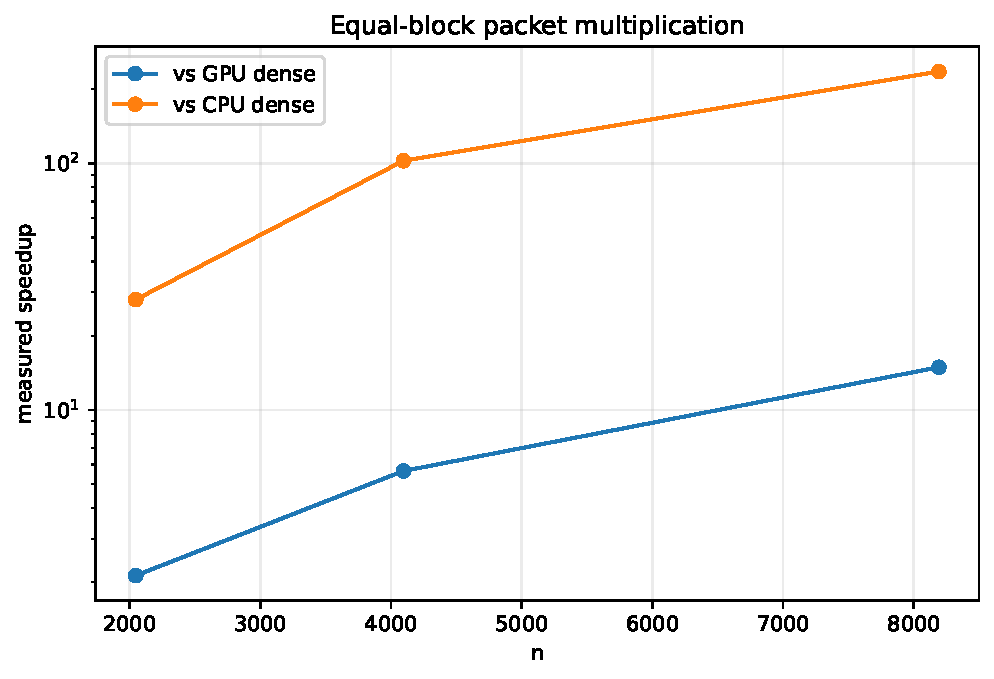
\includegraphics[width=0.78\textwidth]{07_block_diagonal_speedup.pdf}
\caption{Measured speedup of equal-block batched multiplication. The GPU benefit appears only after the mathematical representation has removed the inactive dense blocks.}
\label{fig:block-speedup}
\end{figure}

\subsection{Block diagonal plus low rank}

For $n=8192$, $b=64$, $r=8$, and 32 right-hand sides, the standard PyTorch CUDA packet path took
\[
0.097280\text{ ms},
\]
while CUDA Graph replay took
\[
0.079872\text{ ms}.
\]
The graph-replay row was 10.9355 times faster than GPU dense and 153.6527 times faster than CPU dense, with relative error
\[
3.87\times10^{-7}.
\]
The graph-capture cost was excluded and must be amortized separately.

\begin{figure}[htbp]
\centering
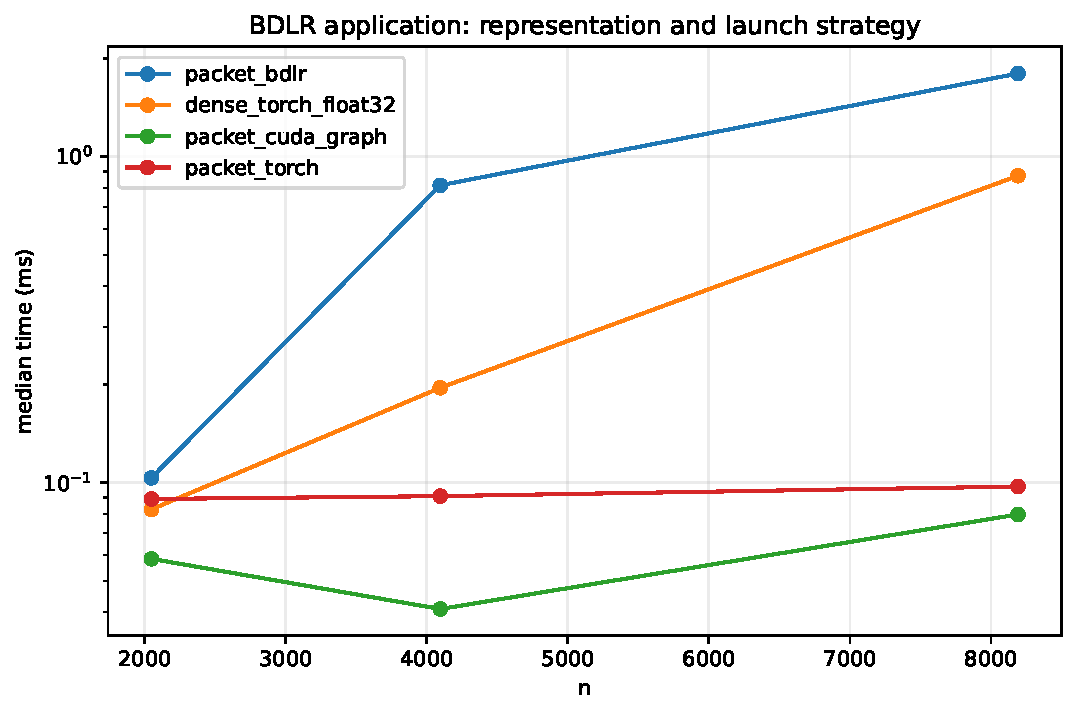
\includegraphics[width=0.82\textwidth]{08_bdlr_timings.pdf}
\caption{Measured BDLR timings. CUDA Graph replay reduces repeated launch overhead for a fixed packet graph.}
\label{fig:bdlr-timings}
\end{figure}

\subsection{Block-banded and sparse transfer graphs}

The block-banded GPU packet path was slower than dense GPU at $n=2048$ but faster at $n=4096$. The sparse-plus-low-rank path showed the same type of crossover. These cases demonstrate that irregular gather/scatter overhead can dominate until enough dense work has been removed.

\subsection{Transforms and tensor operators}

CPU FFT and modewise tensor contractions were competitive or best for several moderate-size vector problems. The $4096$ circulant CPU FFT row was 4.94 times faster than the matched GPU dense row. For Walsh-Hadamard transforms, the CPU was faster at length $65536$, but the GPU became 3.01 times faster than the CPU packet implementation at length $262144$.

\begin{figure}[htbp]
\centering
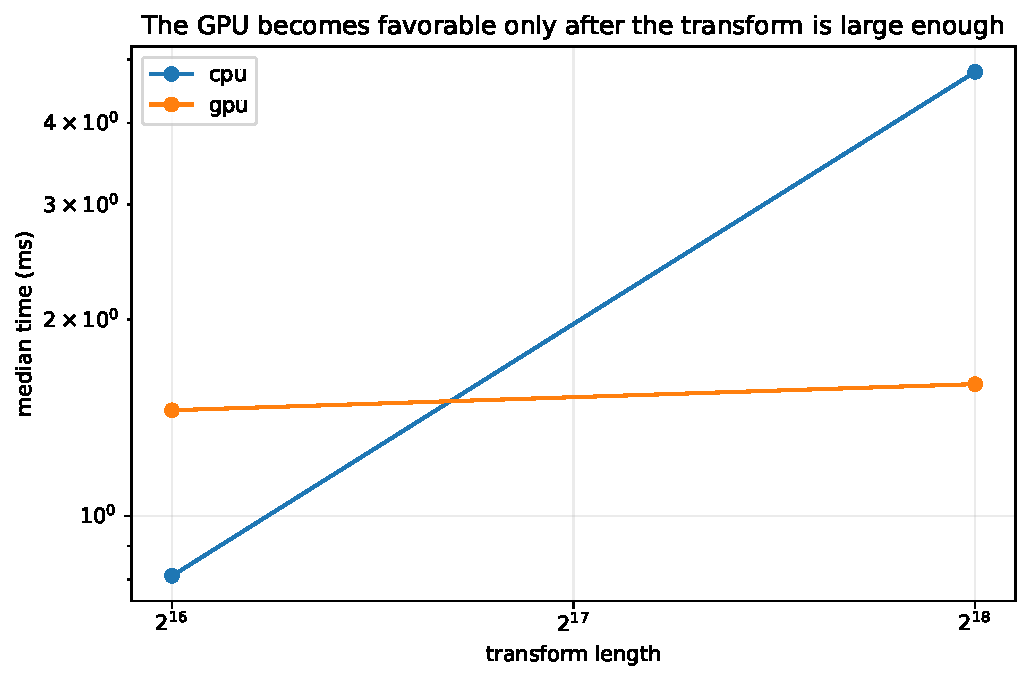
\includegraphics[width=0.78\textwidth]{11_fwht_crossover.pdf}
\caption{Measured Walsh-Hadamard crossover. A GPU launch is not automatically beneficial for every structured transform.}
\label{fig:fwht}
\end{figure}

\begin{figure}[htbp]
\centering
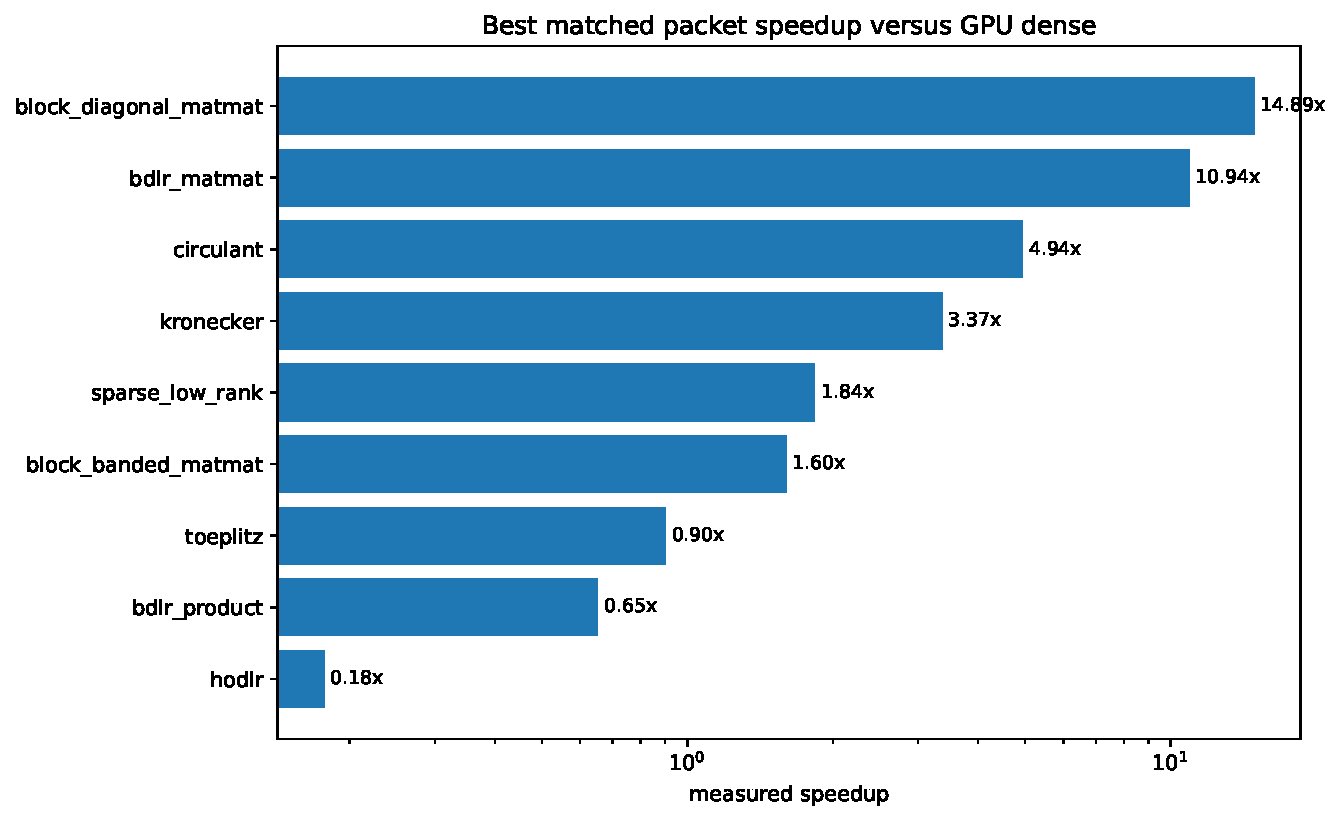
\includegraphics[width=0.88\textwidth]{14_best_packet_speedup_gpu.pdf}
\caption{Best matched packet speedup versus a GPU dense baseline in each eligible suite. Only equal case identifiers and output contracts are used.}
\label{fig:best-gpu}
\end{figure}

\begin{figure}[htbp]
\centering
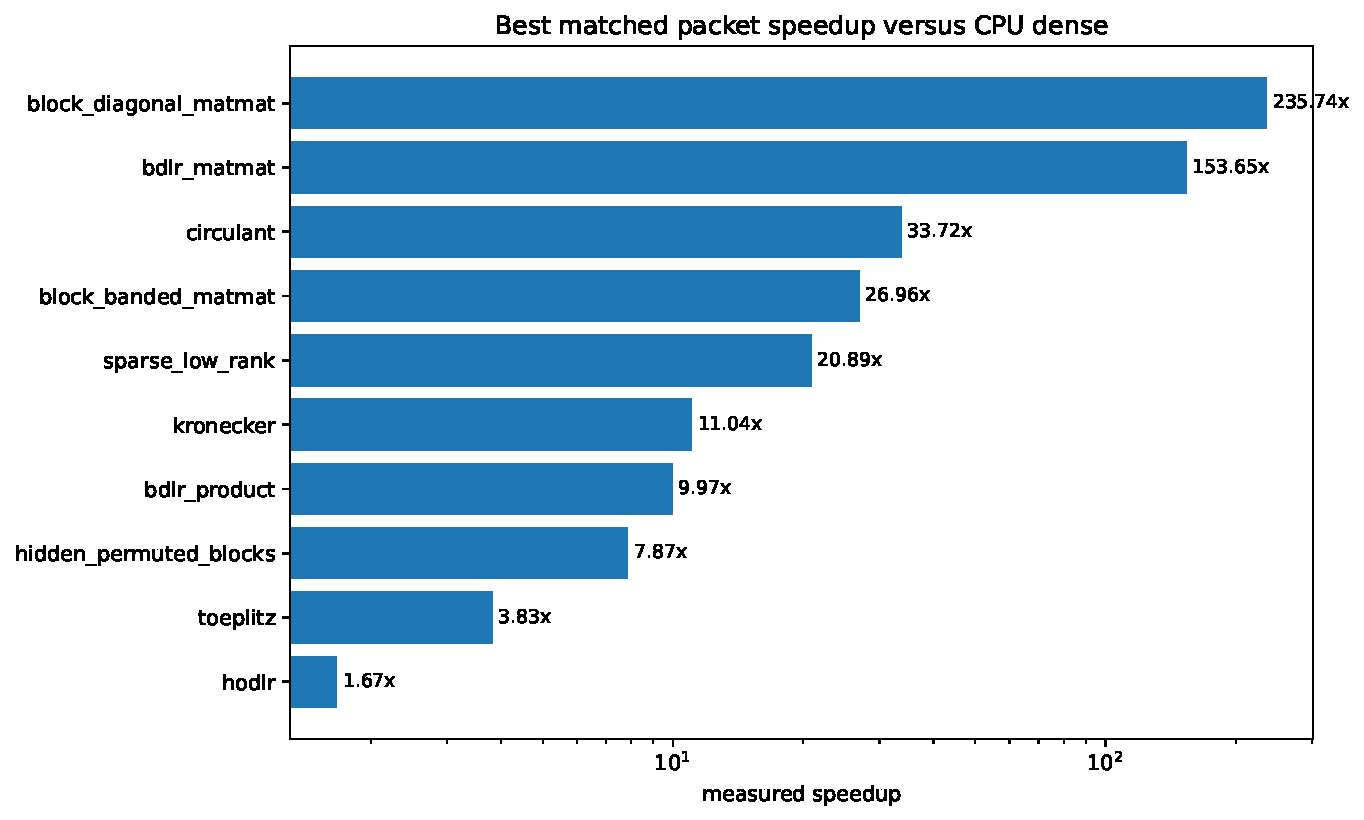
\includegraphics[width=0.88\textwidth]{15_best_packet_speedup_cpu.pdf}
\caption{Best matched packet speedup versus a CPU dense baseline. These numbers combine mathematical work reduction and hardware acceleration.}
\label{fig:best-cpu}
\end{figure}

\section{Discovery, transfer, and reuse}

\subsection{Hidden packet discovery}

For hidden permuted blocks, structure discovery is a one-time cost. At $n=512$, discovery cost $2.1102$ ms, dense application cost $0.0969$ ms, and packet application cost $0.0151$ ms. The exact amortization theorem gives
\[
R_{\min}=26.
\]
At $n=1024$, the corresponding values were $5.2726$, $0.1896$, and $0.0241$ ms, giving
\[
R_{\min}=32.
\]
These match the recorded reuse thresholds.

\begin{figure}[htbp]
\centering
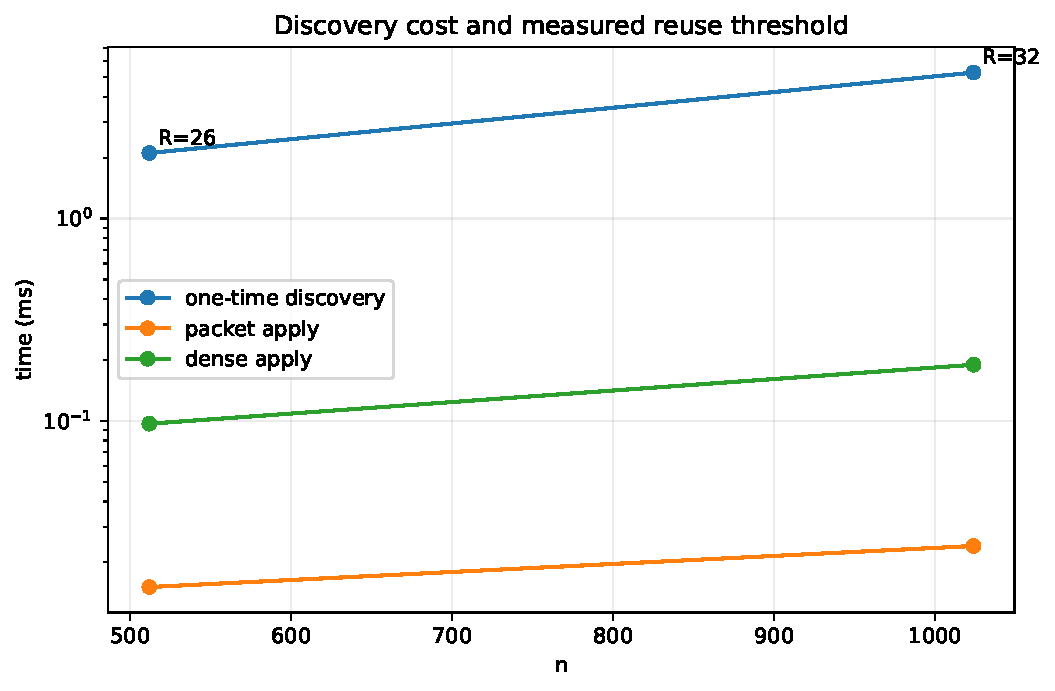
\includegraphics[width=0.78\textwidth]{10_structure_discovery_amortization.pdf}
\caption{Discovery cost is meaningful only together with expected reuse. A structure that is profitable for repeated application may be unprofitable for a single call.}
\label{fig:discovery}
\end{figure}

\subsection{End-to-end transfer}

For a $2048\times2048$ dense FP32 product, CUDA Graph replay took $1.9993$ ms device-resident. The end-to-end pageable path took $7.3036$ ms, while the pinned path took $6.3084$ ms. Two independent dense GEMMs took $3.6557$ ms serially and $4.2368$ ms in the tested two-stream path. The attempted overlap was therefore slower on this hardware and workload.

\begin{figure}[htbp]
\centering
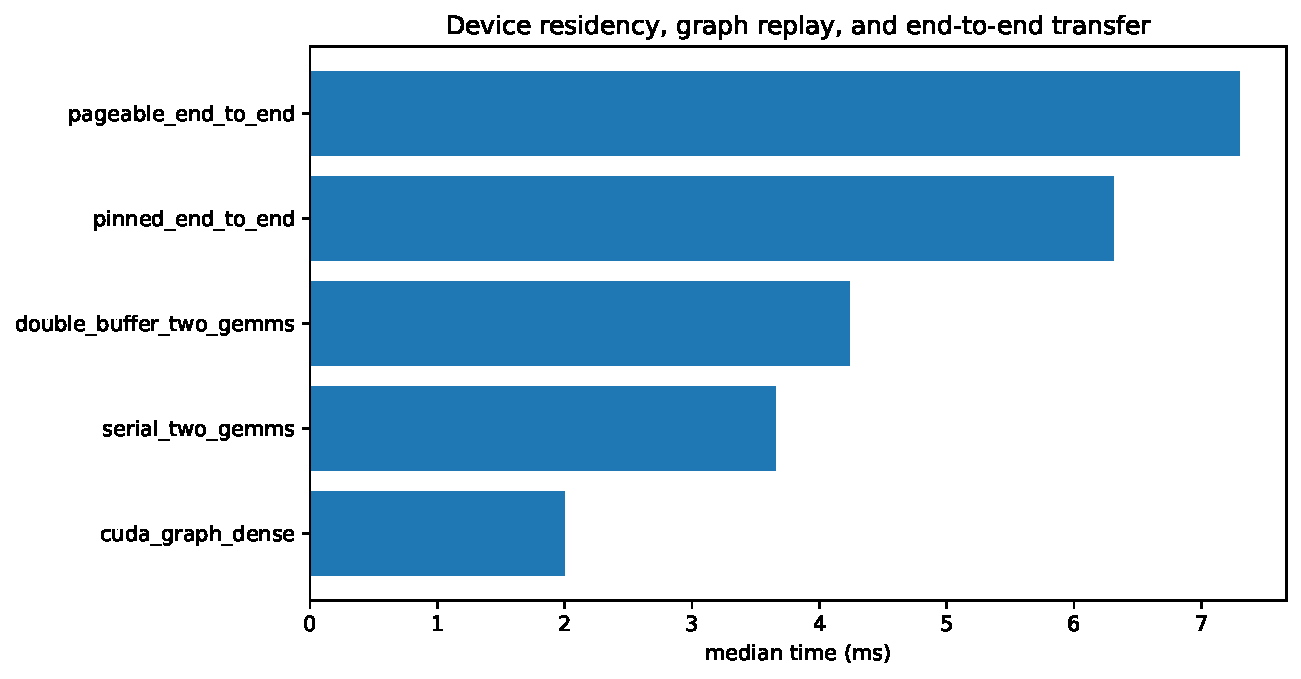
\includegraphics[width=0.84\textwidth]{13_transfer_pipeline.pdf}
\caption{Measured transfer and launch scopes. Device-resident replay, end-to-end execution, and two-output pipelines answer different questions.}
\label{fig:transfer}
\end{figure}

\section{Negative controls and crossover failures}

A benchmark that deletes unfavorable rows cannot distinguish a general method from selective reporting. The following negative results are therefore part of the paper.

\begin{itemize}[leftmargin=1.5em]
\item At $n=512$, recursive Strassen with leaf size 128 took $7.0950$ ms, while OpenBLAS dense multiplication took $1.9597$ ms.
\item At $n=2048$, the tested recursive HODLR GPU path took $5.6079$ ms, while dense GPU multiplication took $0.0860$ ms.
\item The tested FP32 iterative-refinement GPU solve took $22.0848$ ms, while the direct FP64 GPU solve took $12.6286$ ms, with comparable final error.
\item The two-stream dense pipeline was slower than the serial two-GEMM path.
\item The GPU Walsh-Hadamard transform was slower than CPU at length $65536$.
\end{itemize}

\begin{figure}[htbp]
\centering
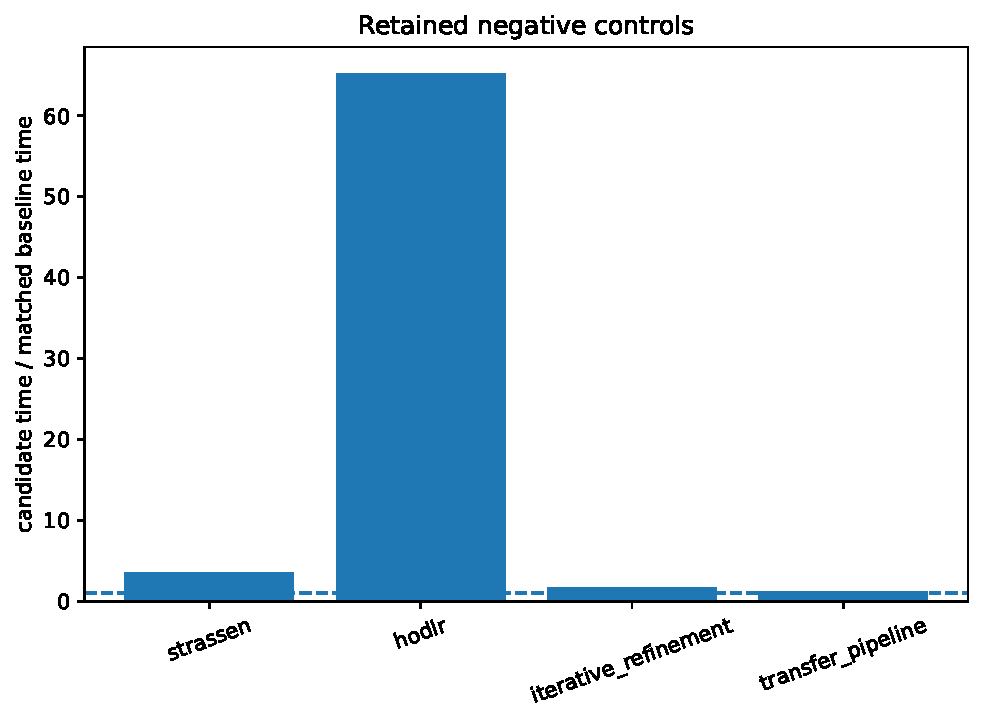
\includegraphics[width=0.80\textwidth]{12_negative_controls.pdf}
\caption{Candidate time divided by matched baseline time. Values above one are slowdowns.}
\label{fig:negative}
\end{figure}

These failures have different causes: recursion overhead, insufficient batch size, small kernel granularity, memory traffic, extra refinement iterations, and limited overlap. They cannot be repaired by one universal implementation rule.

\section{A fair packet benchmark decomposition}

Every speedup can be factored conceptually into four parts:
\[
\boxed{
S_{\mathrm{total}}
 =S_{\mathrm{representation}}
  S_{\mathrm{device}}
  S_{\mathrm{kernel}}
  S_{\mathrm{amortization}}.
}
\]
This expression is interpretive rather than an identity of measured ratios unless each factor is isolated by matched rows. Its purpose is to prevent four distinct questions from collapsing into one number.

\begin{definition}[Representation gain]
The ratio between dense and structured arithmetic or storage for the same mathematical operator, independent of hardware.
\end{definition}

\begin{definition}[Device gain]
The ratio between CPU and GPU time for the same representation, output contract, and timing scope.
\end{definition}

\begin{definition}[Kernel gain]
The ratio between a standard GPU path and a custom, fused, compiled, or graph-replayed path for the same representation.
\end{definition}

\begin{definition}[Amortization factor]
The effect of one-time discovery, transfer, materialization, compilation, or capture costs at a declared reuse count.
\end{definition}

The benchmark corpus contains rows that isolate many, but not all, of these factors. For example, the BDLR suite separates CPU dense, CPU packet, GPU dense, GPU packet, and CUDA Graph replay. The BDLR product suite additionally distinguishes compressed and materialized outputs.

\section{Implementation patterns}

\subsection{Packet BDLR application}

The exact standard implementation is:
\begin{lstlisting}
def apply_bdlr(blocks, u, v, x):
    y = apply_block_diagonal(blocks, x)
    return y + u @ (v.T.conj() @ x)
\end{lstlisting}

On a GPU, equal blocks should be stacked as
\[
(B,b,b)
\]
and right-hand sides as
\[
(B,b,q),
\]
then passed to a batched GEMM. The low-rank term uses two ordinary dense products. A fused custom kernel is useful only if it reduces launch or memory traffic without breaking library-level efficiency.

\subsection{Compressed product pipeline}

When a later stage can consume $(D,U,V)$ directly, the compressed product theorem avoids constructing $n^2$ entries. If an explicit matrix is required, the materialization row must be used. The measured $n=1024$ GPU compressed product took $0.1582$ ms, while materialization took $0.5073$ ms.

\subsection{Packet preconditioned iteration}

The block-diagonal packet part may be factored once and reused. The preconditioner is effective when normalized cross-packet coupling is small. The bound in \cref{thm:preconditioner} does not assert that block Jacobi is always optimal; it provides a verifiable sufficient condition.

\subsection{Mixed precision by packet weight}

A practical policy is:
\begin{enumerate}[leftmargin=1.6em]
\item estimate $\norm{A_e}\norm{P_{\alpha(e)}x}$ or a reusable upper bound;
\item allocate tolerances from the continuous theorem;
\item map tolerances to supported dtypes;
\item accumulate sensitive reductions in a wider type;
\item verify the packet error certificate after reconstruction.
\end{enumerate}

\section{Hardware co-design}

The finite results suggest a packet-native accelerator organized around:
\begin{itemize}[leftmargin=1.5em]
\item grouped small-matrix engines indexed by packet shape;
\item a transfer-graph scheduler;
\item low-rank contraction units;
\item on-chip storage for packet factors rather than materialized matrices;
\item a precision tag on every packet edge;
\item replayable graph descriptors;
\item explicit analysis and synthesis operations.
\end{itemize}

\begin{conjecture}[Packet compiler]
For a declared operator grammar and error tolerance, there exists a compiler that selects a packet partition, support graph, low-rank corrections, precision assignment, and hardware schedule whose total cost is within a controlled factor of the best admissible representation on a specified device model.
\end{conjecture}

\begin{conjecture}[Refinement-stable scheduling]
A nested packet decomposition can be scheduled so that refining one packet changes only its local descendants and incident transfer edges, rather than requiring global recompilation.
\end{conjecture}

\begin{conjecture}[Packet-native memory hierarchy]
For workloads whose operator families remain closed under packet composition and low-rank transfer, storing packet factors through the memory hierarchy can asymptotically reduce data movement relative to repeated dense materialization.
\end{conjecture}

\begin{boundary}[No hardware proof]
The conjectures describe a hardware research program. The current benchmark uses standard CPU and GPU libraries plus CUDA Graph replay. It does not measure a custom packet processor or prove an optimal architecture.
\end{boundary}

\section{Proof, measurement, and claim ledger}

\begin{longtable}{L{0.34\textwidth}L{0.20\textwidth}L{0.37\textwidth}}
\caption{Status of the principal claims.}\label{tab:claims}\\
\toprule
Statement & Status & Boundary\\
\midrule
\endfirsthead
\toprule
Statement & Status & Boundary\\
\midrule
\endhead
Exact packet block reconstruction & Theorem & Finite complete projector systems.\\
Block, sparse, and BDLR counts & Theorem & Modeled arithmetic and representation storage.\\
Compressed BDLR product & Theorem & Same packet partition; no numerical recompression required.\\
Woodbury packet solve & Theorem & Required inverses must exist.\\
Packet preconditioner bound & Theorem & SPD packet part and normalized coupling norm below one.\\
Mixed-precision certificate & Theorem & Declared block operator errors.\\
Precision allocation formula & Theorem & Continuous logarithmic cost model.\\
GPU timing rows & Numerical certificate & Recorded hardware and software only.\\
Universal packet speedup & Rejected & Several tested packet implementations are slower.\\
Improved generic dense exponent & Not claimed & Structure-sensitive and generic dense problems remain separate.\\
Optimal packet compiler & Conjecture & Requires discovery and approximation guarantees.\\
Packet-native accelerator optimality & Conjecture & No custom hardware measured.\\
\bottomrule
\end{longtable}

\section{Verification}

The release contains a sanitized 154-row measured benchmark corpus, derived tables, eighteen figure pairs, exact finite algorithms, and twenty-three automated tests. The current finite verification returned:
\[
\begin{array}{lr}
\text{BDLR apply residual} & 2.74\times10^{-14},\\
\text{Woodbury solve residual} & 1.62\times10^{-15},\\
\text{compressed product residual} & 4.10\times10^{-13},\\
\text{block-sparse apply residual} & 2.52\times10^{-14},\\
\text{mixed-precision actual error} & 1.2614\times10^{-2},\\
\text{mixed-precision certified bound} & 2.4605\times10^{-2},\\
\text{plain CG iterations} & 31,\\
\text{packet-preconditioned CG iterations} & 6.
\end{array}
\]

The sanitized data remove local paths, user-directory strings, raw process listings, and timestamps. The paper source contains no bibliography commands or paper-local references. All visible metadata are restricted to the title, subject, and author name Komorebi P.


\section{Reproducibility and software map}

The release is organized so that the mathematical representation, finite certificates, measured benchmark corpus, and document build remain separable.

\begin{table}[htbp]
\centering
\caption{Implementation map.}
\label{tab:software-map}
\small
\begin{tabularx}{\textwidth}{L{0.27\textwidth}Y}
\toprule
File or module & Role\\
\midrule
\path{packet_gpu/operators.py} & Exact block-diagonal, block-sparse, BDLR, compressed-product, materialization, and Woodbury operations.\\
\path{packet_gpu/complexity.py} & Arithmetic, storage, intensity, launch-count, and amortization formulas.\\
\path{packet_gpu/mixed_precision.py} & Packet error certificates, quantization tests, and continuous tolerance allocation.\\
\path{packet_gpu/krylov.py} & Conjugate gradient, packet preconditioning, and finite Lanczos certificates.\\
\path{packet_gpu/benchmark_data.py} & Sanitization, fairness audit, summary tables, negative controls, and matched speedup extraction.\\
\path{packet_gpu/visuals.py} & Eighteen reproducible figure pairs.\\
\path{data/benchmark_results_sanitized.json} & Measured 154-row CPU/GPU corpus with private paths and timestamps removed.\\
\path{results/paper_viii_results.json} & Finite certificate and corpus summary used by the paper.\\
\path{tests/} & Twenty-three correctness, complexity, fairness, mixed-precision, Krylov, and figure-generation tests.\\
\bottomrule
\end{tabularx}
\normalsize
\end{table}

The core BDLR application has four stages:
\[
\boxed{
X
\longmapsto
DX
\longmapsto
V^*X
\longmapsto
U(V^*X)
\longmapsto
DX+U(V^*X).
}
\]
A correct GPU implementation may fuse stages or change their schedule, but it must preserve this mathematical contract. The benchmark records the dense-equivalent logical work and the modeled executed work separately. Logical GFLOP/s may therefore exceed the physical dense throughput when the packet representation avoids most of the dense arithmetic; it is a work-equivalence statistic, not a claim that those dense operations were executed.

The PowerShell runner checks for installed packages before invoking \texttt{pip}. Dependencies are installed only when missing, unless the explicit \texttt{-Update} switch is supplied. The runner regenerates finite results and figures, executes the tests, builds the wheel, and compiles the paper when \texttt{latexmk} is available. It does not silently replace a working CUDA installation or claim a new GPU measurement.

\section{Conclusion}\label{sec:conclusion}

The computational realization of the seed calculus begins before CUDA. The first decision is the mathematical representation:
\[
A=\sum_{\alpha,\beta}P_\beta AP_\alpha.
\]
When most blocks vanish or admit low-rank transfer, arithmetic and storage can fall from dense $n^2$ scaling to a structure-sensitive count. Hardware then determines how much of that reduction becomes wall-clock gain.

The measured corpus supports four conclusions. First, equal regular packets and BDLR operators can substantially outperform matched dense CPU and GPU baselines. Second, device residency and launch amortization matter enough to change the ranking. Third, output contracts must be respected: compressed factors and explicit matrices are different products. Fourth, packet structure is not a universal guarantee of speed. Irregular recursion, small transforms, discovery costs, transfer, and additional refinement steps can erase or reverse the gain.

The common operator language therefore yields a disciplined computational principle:
\[
\boxed{
\begin{gathered}
\text{remove work by representation},\\
\text{map regular packets to batched hardware},\\
\text{assign precision by packet sensitivity},\\
\text{amortize discovery and transfer explicitly},\\
\text{retain negative controls},\\
\text{reconstruct the declared output exactly or within a certified error}.
\end{gathered}
}
\]

This is the computational bridge from the abstract seed calculus to practical dense, structured, iterative, and GPU algorithms. The next paper returns to arithmetic: Euler families, supercongruences, and weighted $p$-adic reconstruction.

\end{document}
